\documentclass[a4paper, pt14]{article}

\usepackage[utf8]{inputenc}
\usepackage[T1]{fontenc}
\usepackage[slovene]{babel}
\usepackage{lmodern}
%\usepackage{hyperref}
\usepackage{amsmath}
\usepackage{amssymb}
\usepackage{graphicx}
\usepackage{listings}


\begin{document}

\title{%
Scheduling-Queues\\
  \large Finančni praktikum}
\author{Špela Bernardič, Ioann Stanković}
\date{10. \ 1. \ 2023}

\maketitle






\section{Navodilo naloge}
Naloga se ukvarja z algoritmi 'Scheduling-Queues', ki uporabljajo podatke napovedane s strojnim učenjem.
Potrebno je napisati simulacijo procesov, ki uporabi napovedane čase trajanja procesov in nato narediti analizo časa čakanja procesov.
Preveriti je potrebno, kako različene porazdelitve trajanja procesov in kvaliteta napovedi vplivata na povprečen čas čakanja v vrsti.
Napovedi časov trajanja procesov se lahko določi z dodajanjem šumov pravim vrednostim, lahko pa se uporabi naučen model.


\section{Opis problema}

S problemom razvrščanja opravil v vrsti se srečamo na različnih področjih. Za opravila nevemo nujno njihove dolžino trajanja, velikokrat pa jo laho ocenimo oziroma napovemo. 
Zato je poleg optimalnosti algoritmov, ki za razvrščanje uporabljajo dejanske čase trajanja opravila, smiselno analizirati tudi primere, ko se uporabljajo napovedani časi trajanja opravila.
Opazovati je torej treba (povprečen) čas čakanja opravila v vrsti. Želimo, da je ta čim krajši.

\section{Algoritmi razvrščanja procesov}

Za reševanje problema razvrščanja procesov v vrsti se uporabljaj različni algoritmi. V nalogi sva uporabila naslednje osnovne algoritme:
\begin{itemize}
  \item FCFS (First Come First Serve) je algoritem, ki izvaja procese po vrstnem redu njihovega prihoda.
  \item SJF (Non-Preemptive Shortest Job First) je algoritem, pri katerem se za naslednjo izvedbo izbere proces z najkrajšim časom trajanja. Ko se določi kateri proces se naj izvede naslednji, se ta izvede do konca. 
  \item PSJF (Preemptive Shortest Job First) je algoritem, pri katerem se proces z najkrajšim časom trajanja začne izvajati prvi. Ob prihodu novega procesa se le ta postavi v čakalno vrsto. Če pa pride proces s krajšim trajanjem od procesa, ki se trenutno izvaja, se trenutni proces ustavi in vrne v vrsto. Začne se izvajati proces s krajšim trajanjem.
  \item SRPT (Shortest remaining processing time) je algoritem podoben PSJF, vendar ta upošteva preostanke trajanj procesov.
\end{itemize}

Poleg osnovnih algoritmov sva napisala še variacje z napovedmi:

\begin{itemize}
  \item SPJF (Non-Preemptive Shortest Predicted Job First) za naslednjo izvedbo izbere proces z najkrajšim \textbf{napovedanim} časom trajanja. 
  \item PSPJF (Preemptive Shortest Predicted Job First) razvršča procese glede na najkrajši \textbf{napovedan} čas trajanja.
  \item SPRPT (Shortest Predicted remaining processing time) je algoritem podoben PSPJF, vendar ta upošteva preostanek \textbf{napovedanega} trajanj procesov.
\end{itemize}

Primer enega od algoritmov:

\begin{verbatim}

def PSPJF(seznam):
  opravila = sorted((Opravilo(*t) for t in seznam), key=lambda item: item.arrival)
  opravila = + [Opravilo(None, float('inf'), float('inf'), float('inf'))] 
  vrsta = []
  t = 0
  cakanje = 0
  for naslednje in opravila:
      while vrsta: 

          prekinitev = naslednje.arrival - t 
          if prekinitev <= 0:
              break 

          predvideno, cas, opravilo = vrsta[0]
          preostanek = cas - prekinitev

          if preostanek > 0:
              if predvideno > naslednje.predicted:
                  vrsta[0] = (predvideno, preostanek, opravilo) 
                  t = naslednje.arrival
                  break 

              else:  
                  break

          else:
              heappop(vrsta)
              t += cas
              cakanje += t - opravilo.length - opravilo.arrival
      else:
          t = naslednje.arrival 
      
      heappush(vrsta, (naslednje.predicted, naslednje.length, naslednje)) 
  return cakanje 
\end{verbatim}

\section{Generiranje podatkov}
Za algoritme je bilo potrebno zgenerirat podatke za čase prihodov opravil, dolžine teh opravil, in šum na opravilih. 
Za generiranje podatkov sva uporabila programski jezik R. Čase prihodov opravil sva zgenerirala z eksponentno porazdelitvijo s parametrom $\lambda = 0.25$, torej $N \sim exp(0.25) $. 
Dolžino opravil sva generirala z beta in normalno porazdelitvijo.
Šum pa sva dodala z normalno porazdelitvijo $ Z \sim N(0, 0.01) $. 
Želela sva analizirati, kako se čas čakanja spremeni glede na kvaliteto napovedi. Zato sva šum zgenerirala za $ Z \sim N(0, \sigma) $ pri različnh $\sigma$.
Da bi se izognila dolžinam opravil in šumu velikosti 0 sva za minimalno dolžino opravila vzela $10^{-7}$. Da bi bili končni podatki bolj relevantni, sva poskuse izvajala po 100-krat in na koncu pri vzela povprečje razltatov.

\subsection{Generiranje dolžin opravil Normalne porazdelitve}
Za generiranje dolžin opravil sva v enem primeru sva uporabila Normalno porazdelitev $Y \sim |N(5,5)|$, vzela sva absolutno vrednost normalne porazdelitve, da bi se izognila negativnim vrednostim. Po izra\v cunu $ \mu_Y = \sqrt{\sigma \frac{2}{\pi}} e^{-\frac{\mu^2}{2\sigma}} + \mu [1- \Phi(-\frac{\mu}{\sqrt{\sigma}})] $ in $ \sigma^2_Y = \mu^2 + \sigma^2 - \mu^2_Y $, je $E[Y] = 3.559897$ in $ Var[Y] = 17.32713$. 

\subsection{Generiranje dolžin opravil Beta porazdelitve}
V drugem primeru pa beta porazdelitev skalirano za 10, torej $X \sim Beta(\alpha, \beta) \times 10 $, s pričakovano vrednostjo $ E[X] = 5$ in varianco $Var[X] = 1 $. Od tod sva izračunala parametre za beta porazdelitev $\alpha = \beta = 12$.\\
Zanimalo naju je tudi, če se oblika grafa čakanja spremeni, ko izberemo majhne dolžine opravil. To sva opazovala le za Beta porazdelitev. Izbrala sva si vrednosti za porazdelitev dolžine opravil $E[X] = 0.5$ in $Var[X] = 0.01 $ (torej $X \sim Beta(12,12)$) ter določila šum z $Var[Z] = 0.01 $.

\section{Analiza}

\subsection{Analiza |N(5,5)| porazdelitve}

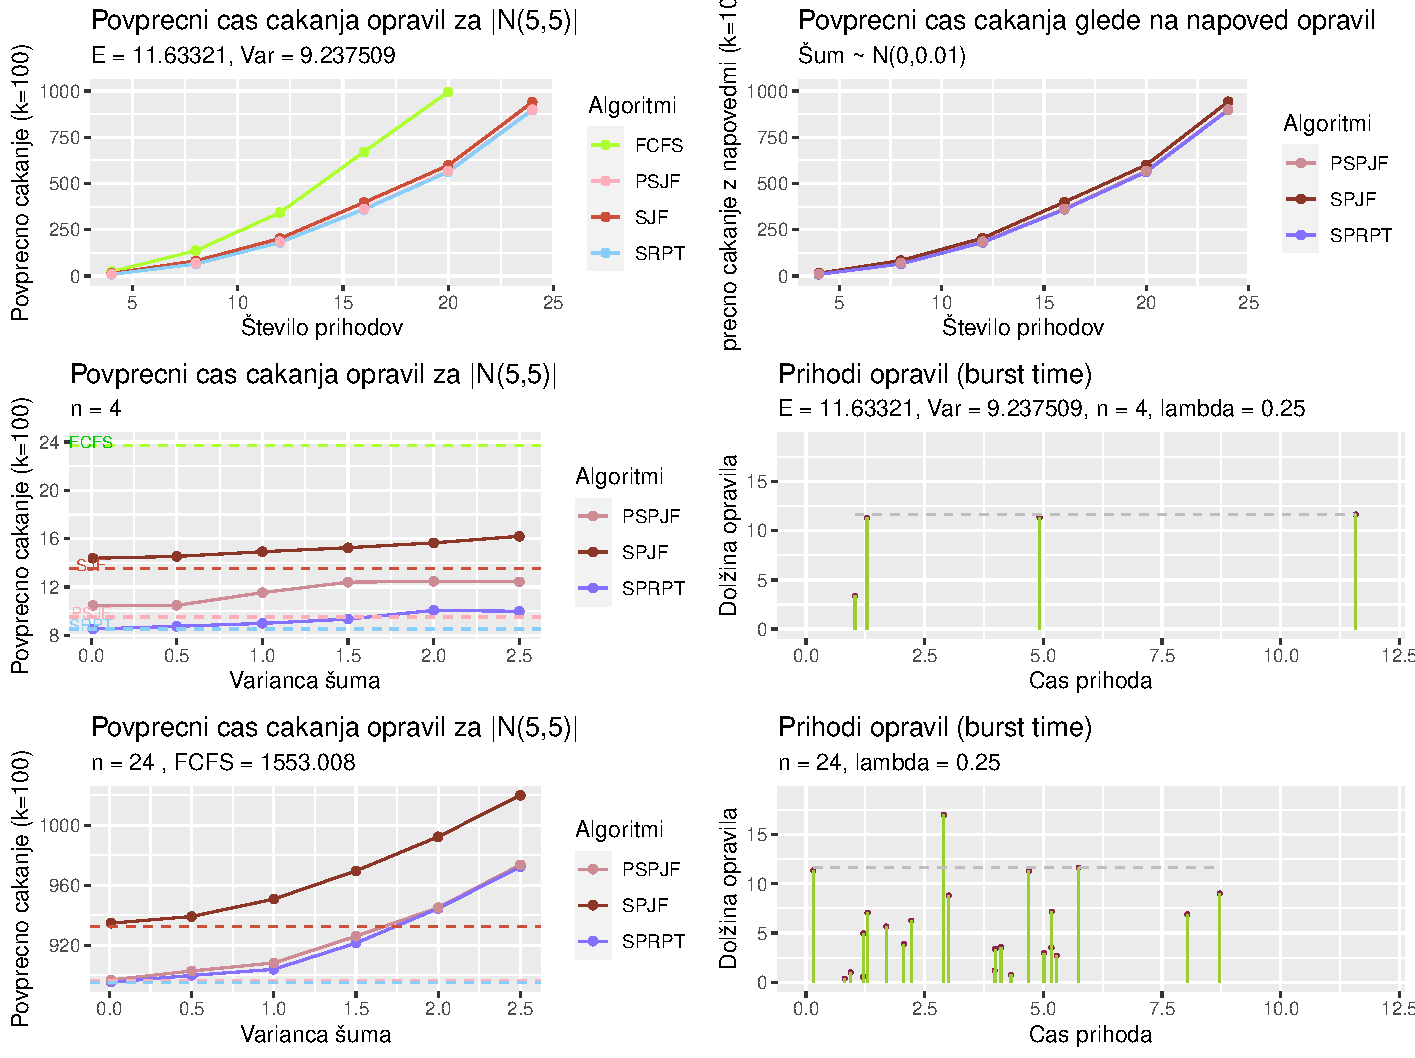
\includegraphics[width=12.1cm,keepaspectratio]{Normalna_grafi.pdf}
\\Iz grafov lahko sklepamo, da čas povprečnega čakanja narašča eksponentno glede na število prihodov. Opazimo večje odstopanje pri algoritmu FCFS, to pripišemo večji varianci podatkov, torej večja kot je varianca podatkov, večje je odstopanje med razvrstitvenimi algoritmi, najbolj opazno pri FCFS, v tem primeru lahko kratka opravila čakajo dolgo časa.

\subsection{Analiza Beta(12,12)$\cdot 10$ porazdelitve}
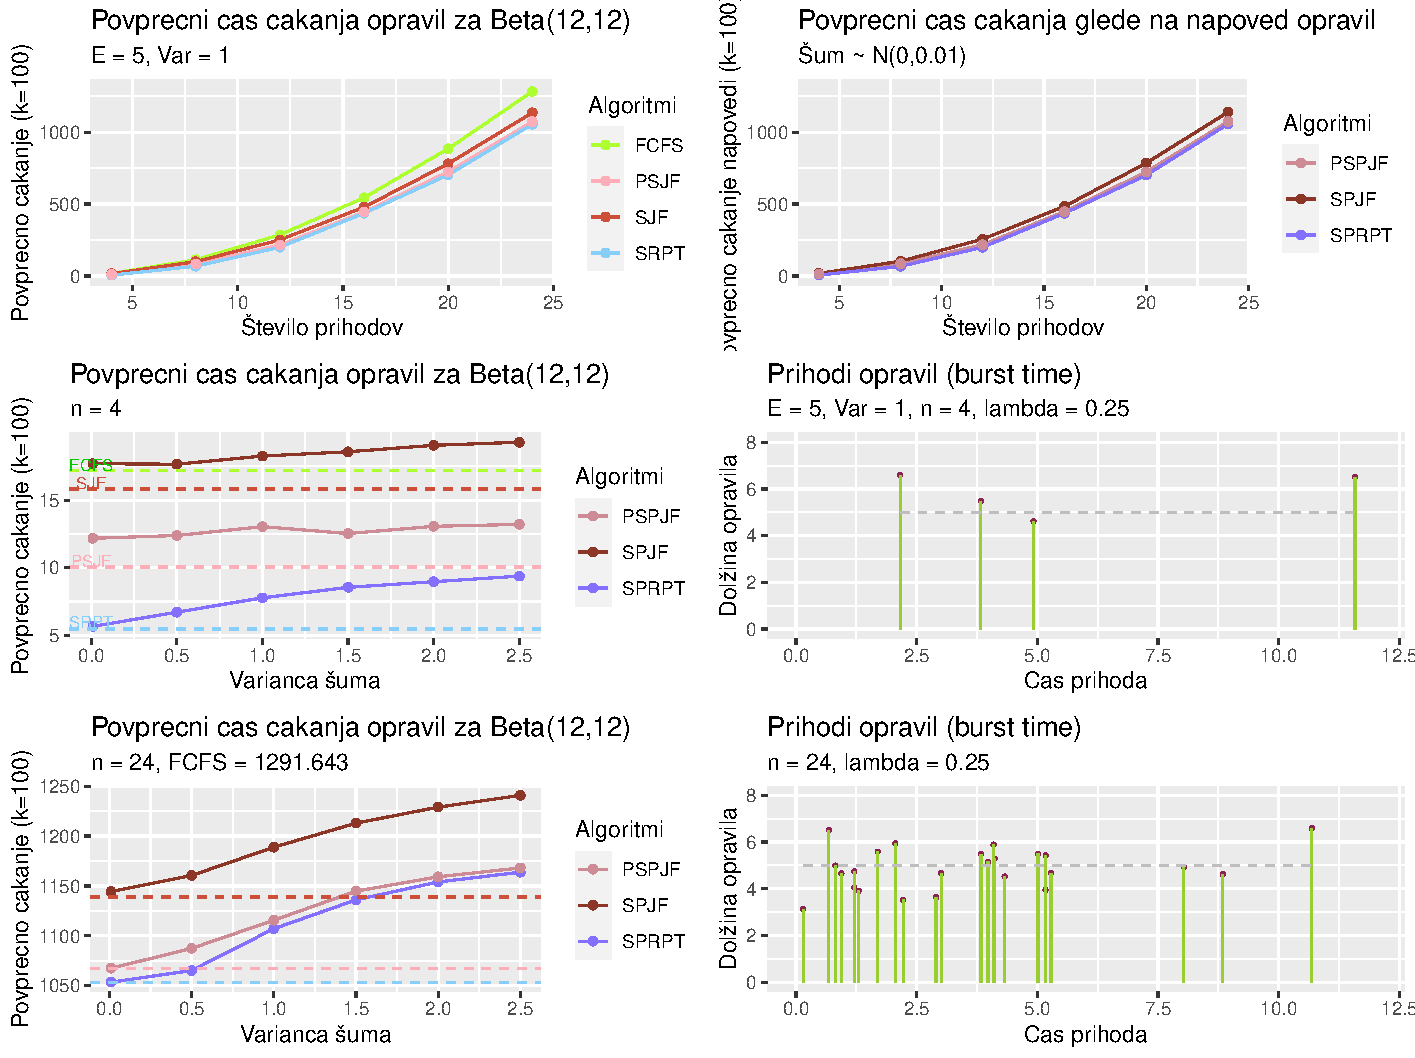
\includegraphics[width=12.1cm,keepaspectratio]{Beta_grafi.pdf}
\\ Imamo podobna opažanja kot pri prvem primeru. Vendar presenetljiv rezultat je, da za majhno število prihodov (v našem primeru n=4) je algoritem FCFS hitrejši kot PSJF, kar za večje število prihodov ne velja. Torej lahko se zgodi, da za majhno število prihodov algoritem PSJF ni najbolj učinkovit. Prav tako je zanimivo opažanje da se s povečevanjem šuma  učinkovitost algoritmov z napovedmi poslabša, torej večji kot imamo šum slabše delujejo algoritmi z bolj učinkovitim razvrščanjem, opazimo da se za velik šum bolj splača uporabljati algoritem SPJF kot SPRPT. Za več prihodov pa postane PSPJF počasnejši kot SPJF. To velja za majhne variance dolžin opravil. Iz grafov sklepava, da povprečni čas čakanja narašča linearno s spremembo variance šuma. Nisva pogledala obnašanje algoritmov za večje variance šumov, saj se nam to ni zdelo smiselno.\\
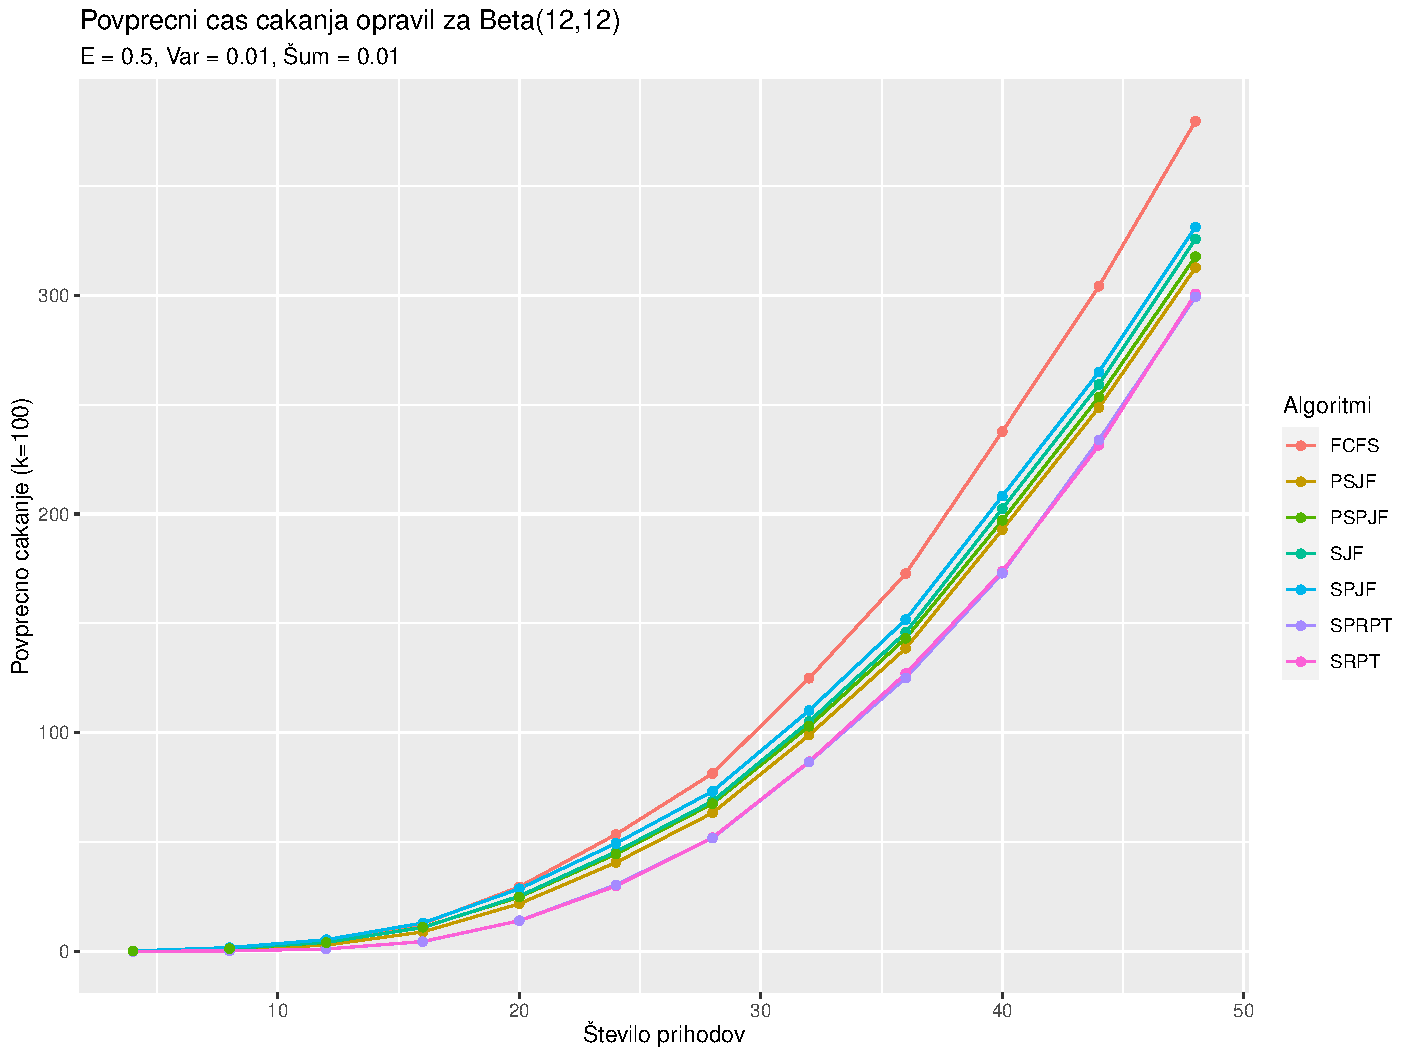
\includegraphics[width=12.1cm,keepaspectratio]{Beta_grafi_majhna.pdf}
\\
Zanimalo nas je, če bodo odstopanja med algoritmi večja, če zmanjšamo pričakovani čas dolžin opravil. Vendar temu ni bilo tako, vidimo da res varianca vpiva na odstopanje med algoritmi. 

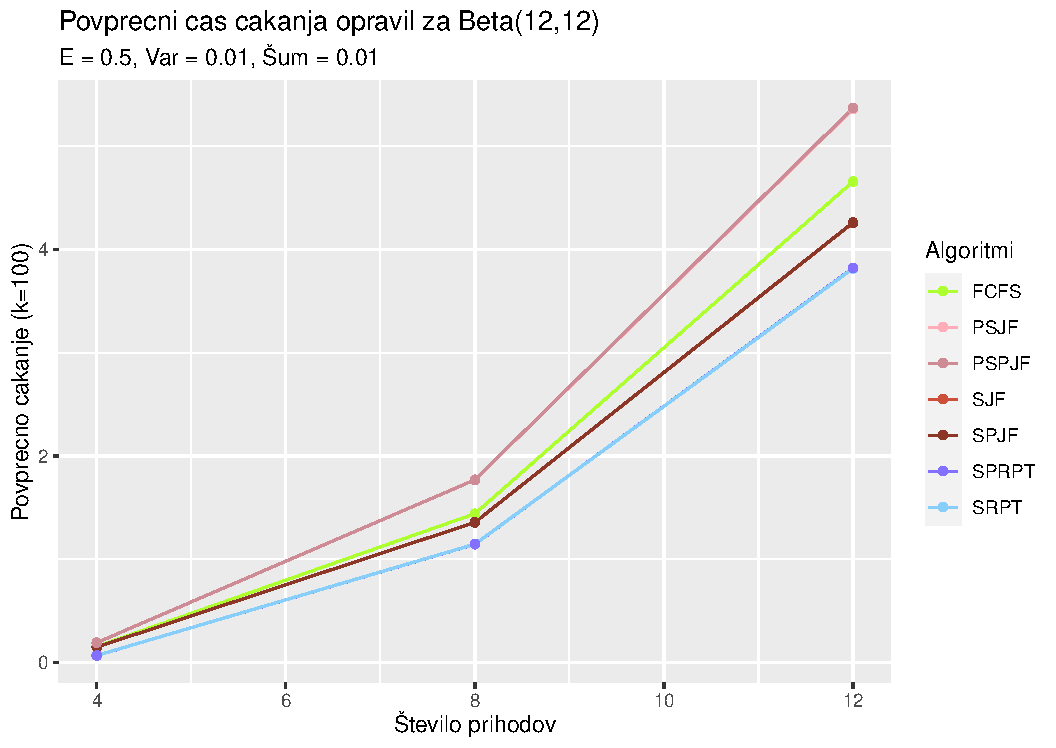
\includegraphics[width=12.1cm,keepaspectratio]{Beta_grafi_razclenitev1.pdf}
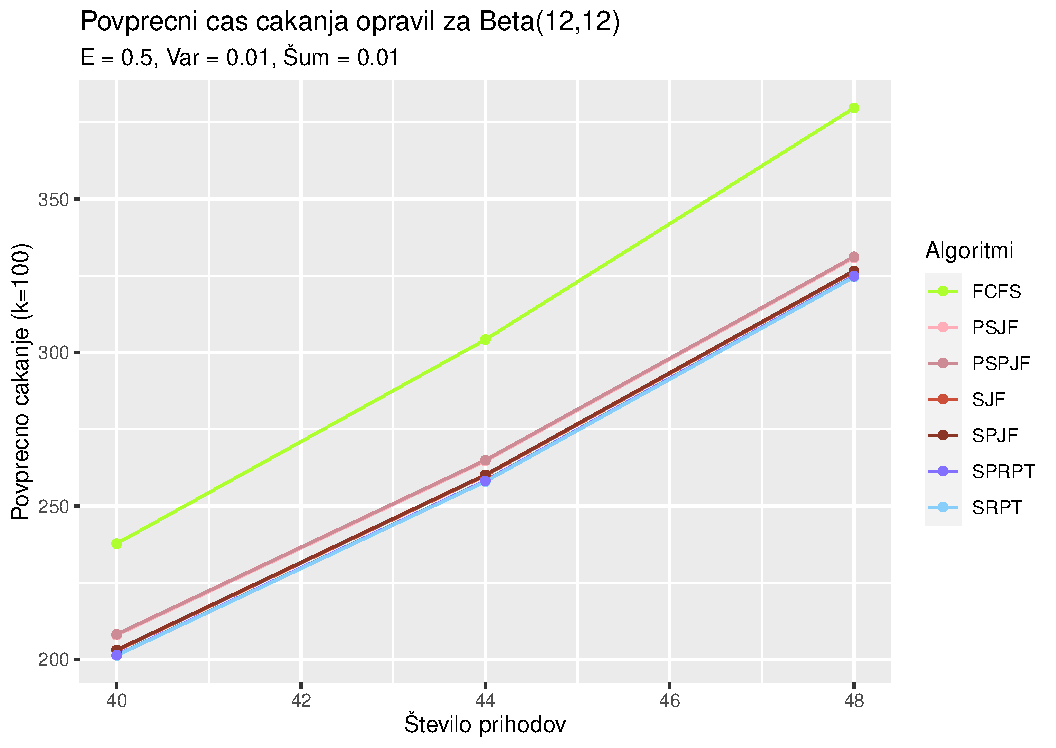
\includegraphics[width=12.1cm,keepaspectratio]{Beta_grafi_razclenitev2.pdf}
\\Vidimo, da četudi imamo neke podatke, kjer je FCFS hitrejši kot PSPJF za malo prihodov, za več prihodov opravil ni več tako, in FCFS postane znatno počasnejši. To da je algoritem FCFS hitrejši kot PSJF pripišemo manjši varianci dolžin opravil.

\subsection{Ugotovitve}
Če je naš cilj minimizirati povprečni čas čakanja opravil se nam zagotovo splača uporabiti algoritem SRPT, če imamo dokaj točne napovedi dolžin uporabimo SRPT z napovedmi (SPRPT). Če pa nimamo najbolj točnih podatkov za dolžine opravil, torej imamo velik šum na podatkih, se na podlagi začetne variance dolžin opravil odločimo, kateri algoritem uporabimo. Večja kot je varianca dolžin opravil, večji šum si lahko privoščimo.
 
\end{document}